% This is "sig-alternate.tex" V2.0 May 2012
% This file should be compiled with V2.5 of "sig-alternate.cls" May 2012
%
% This example file demonstrates the use of the 'sig-alternate.cls'
% V2.5 LaTeX2e document class file. It is for those submitting
% articles to ACM Conference Proceedings WHO DO NOT WISH TO
% STRICTLY ADHERE TO THE SIGS (PUBS-BOARD-ENDORSED) STYLE.
% The 'sig-alternate.cls' file will produce a similar-looking,
% albeit, 'tighter' paper resulting in, invariably, fewer pages.
%
% ----------------------------------------------------------------------------------------------------------------
% This .tex file (and associated .cls V2.5) produces:
%       1) The Permission Statement
%       2) The Conference (location) Info information
%       3) The Copyright Line with ACM data
%       4) NO page numbers
%
% as against the acm_proc_article-sp.cls file which
% DOES NOT produce 1) thru' 3) above.
%
% Using 'sig-alternate.cls' you have control, however, from within
% the source .tex file, over both the CopyrightYear
% (defaulted to 200X) and the ACM Copyright Data
% (defaulted to X-XXXXX-XX-X/XX/XX).
% e.g.
% \CopyrightYear{2007} will cause 2007 to appear in the copyright line.
% \crdata{0-12345-67-8/90/12} will cause 0-12345-67-8/90/12 to appear in the copyright line.
%
% ---------------------------------------------------------------------------------------------------------------
% This .tex source is an example which *does* use
% the .bib file (from which the .bbl file % is produced).
% REMEMBER HOWEVER: After having produced the .bbl file,
% and prior to final submission, you *NEED* to 'insert'
% your .bbl file into your source .tex file so as to provide
% ONE 'self-contained' source file.
%
% ================= IF YOU HAVE QUESTIONS =======================
% Questions regarding the SIGS styles, SIGS policies and
% procedures, Conferences etc. should be sent to
% Adrienne Griscti (griscti@acm.org)
%
% Technical questions _only_ to
% Gerald Murray (murray@hq.acm.org)
% ===============================================================
%
% For tracking purposes - this is V2.0 - May 2012

\documentclass{sig-alternate}
\usepackage{fixltx2e}
\usepackage{xcolor}
\usepackage{amsmath,array}
\usepackage{multirow}
\newcolumntype{L}[1]{>{\raggedright\arraybackslash}m{#1}}
\def\SPSB#1#2{\rlap{\textsuperscript{\textcolor{red}{#1}}}\SB{#2}}
\def\SP#1{\textsuperscript{\textcolor{black}{#1}}}
\def\SB#1{\textsubscript{\textcolor{black}{#1}}}
\newenvironment{myquote}
               {\list{}{\rightmargin   \leftmargin
                        \parsep        0in }%
                \item\relax}
               {\endlist}
\newcommand{\userquote}[2]{\begin{samepage}\begin{myquote} 
     \em{\small{#2\begin{flushright}---#1\end{flushright}}}
   \end{myquote}\end{samepage}}
%Quote code
%\newif\ifquoteopen
%\catcode`\"=\active % lets you define `"` as a macro
%\DeclareRobustCommand*{"}{%
%   \ifquoteopen
%     \quoteopenfalse ''%
%   \else
%     \quoteopentrue ``%
%   \fi
%}

%End of quote code

\begin{document}
\setlength{\parindent}{0pt}
%\CopyrightYear{2016}
\setcopyright{acmcopyright}
\conferenceinfo{ACM DEV '16,}{Nov 18-21, 2016, Nairobi, Kenya}
%\isbn{978-1-4503-4306-0/16/06}\acmPrice{\$15.00}
%\doi{http://dx.doi.org/10.1145/2909609.2909664}
%
% --- Author Metadata here ---
%\conferenceinfo{ICTD'16}{June 3-6 2016, Ann Arbor, Michigan, USA}
%\CopyrightYear{2007} % Allows default copyright year (20XX) to be over-ridden - IF NEED BE.
%\crdata{0-12345-67-8/90/01}  % Allows default copyright data (0-89791-88-6/97/05) to be over-ridden - IF NEED BE.
% --- End of Author Metadata ---

%\title{Alternate {\ttlit ACM} SIG Proceedings Paper in LaTeX
%\title{Leveraging on Families' Social Interactions on Utilization of Personal Health Informatics through Intermediaries}
\title{A Family Health App: Engaging Children to Manage Wellness of Adults}
%
% You need the command \numberofauthors to handle the 'placement
% and alignment' of the authors beneath the title.
%
% For aesthetic reasons, we recommend 'three authors at a time'
% i.e. three 'name/affiliation blocks' be placed beneath the title.
%
% NOTE: You are NOT restricted in how many 'rows' of
% "name/affiliations" may appear. We just ask that you restrict
% the number of 'columns' to three.
%
% Because of the available 'opening page real-estate'
% we ask you to refrain from putting more than six authors
% (two rows with three columns) beneath the article title.
% More than six makes the first-page appear very cluttered indeed.
%
% Use the \alignauthor commands to handle the names
% and affiliations for an 'aesthetic maximum' of six authors.
% Add names, affiliations, addresses for
% the seventh etc. author(s) as the argument for the
% \additionalauthors command.
% These 'additional authors' will be output/set for you
% without further effort on your part as the last section in
% the body of your article BEFORE References or any Appendices.

\numberofauthors{3} %  in this sample file, there are a *total*
% of EIGHT authors. SIX appear on the 'first-page' (for formatting
% reasons) and the remaining two appear in the \additionalauthors section.
%
\author{
% You can go ahead and credit any number of authors here,
% e.g. one 'row of three' or two rows (consisting of one row of three
% and a second row of one, two or three).
%
% The command \alignauthor (no curly braces needed) should
% precede each author name, affiliation/snail-mail address and
% e-mail address. Additionally, tag each line of
% affiliation/address with \affaddr, and tag the
% e-mail address with \email.
%
% 1st. author
%\alignauthor
%        Ntwa Katule \\
%        \affaddr{University of Cape Town}\\
%        \affaddr{Department of Computer Science}\\
%        \affaddr{Cape Town, South Africa}\\
%        \email{katulentwa@gmail.com}
% 2nd. author
%\alignauthor
%Melissa Densmore\\
%        \affaddr{University of Cape Town}\\
%        \affaddr{Department of Computer Science}\\
%        \affaddr{Cape Town, South Africa}\\
        %\affaddr{Institute for Clarity in Documentation}\\
        %\affaddr{P.O. Box 1212}\\
        %\affaddr{Dublin, Ohio 43017-6221}\\
%        \email{mdensmore@cs.uct.ac.za}
% 3rd. author
%\alignauthor Ulrike Rivett\\
%        \affaddr{University of Cape Town}\\
%        \affaddr{Department of Information Systems}\\
%        \affaddr{Cape Town, South Africa}\\
%        \email{ulrike.rivett@uct.ac.za}
       %\affaddr{The Th{\o}rv{\"a}ld Group}\\
        %\affaddr{1 Th{\o}rv{\"a}ld Circle}\\
        %\affaddr{Hekla, Iceland}\\
        %\email{larst@affiliation.org}
%\and  % use '\and' if you need 'another row' of author names
% 4th. author
%\alignauthor Lawrence P. Leipuner\\
%       \affaddr{Brookhaven Laboratories}\\
%       \affaddr{Brookhaven National Lab}\\
%       \affaddr{P.O. Box 5000}\\
%       \email{lleipuner@researchlabs.org}
% 5th. author
%\alignauthor Sean Fogarty\\
%       \affaddr{NASA Ames Research Center}\\
%       \affaddr{Moffett Field}\\
%       \affaddr{California 94035}\\
%       \email{fogartys@amesres.org}
% 6th. author
%\alignauthor Charles Palmer\\
%       \affaddr{Palmer Research Laboratories}\\
%       \affaddr{8600 Datapoint Drive}\\
%       \affaddr{San Antonio, Texas 78229}\\
%       \email{cpalmer@prl.com}
}
% There's nothing stopping you putting the seventh, eighth, etc.
% author on the opening page (as the 'third row') but we ask,
% for aesthetic reasons that you place these 'additional authors'
% in the \additional authors block, viz.
%\additionalauthors{Additional authors: John Smith (The Th{\o}rv{\"a}ld Group,
%email: {\texttt{jsmith@affiliation.org}}) and Julius P.~Kumquat
%(The Kumquat Consortium, email: {\texttt{jpkumquat@consortium.net}}).}
\date{30 July 1999}
% Just remember to make sure that the TOTAL number of authors
% is the number that will appear on the first page PLUS the
% number that will appear in the \additionalauthors section.

\maketitle 

\begin{abstract} 
The pandemic of lifestyle-related chronic diseases has led to an advent of personal health informatics, with the goal of persuading individuals to adopt healthful lifestyles. Such systems implement various motivational strategies to promote ongoing use. Existing initiatives to design such systems focus on engaging only the beneficiary of information derived from those systems. In this study, we explored how one can use gamification to motivate ongoing usage of such systems in the context of intermediated technology use. We studied the effect of gamification in motivating young family members to assist adults who might be less conversant or intimidated with such a technology. We compared two designs of a mobile wellness application of which one prototype is gamified and the other one is not gamified. Our findings suggest that virtual rewards can enhance usage of such systems through intermediary users. We highlight some of the design implications in order to foster perceived enjoyment in using such a system.    
\end{abstract}
%
% The code below should be generated by the tool at
% http://dl.acm.org/ccs.cfm
% Please copy and paste the code instead of the example below. 
%

\begin{CCSXML}
<ccs2012>
<concept>
<concept_id>10002944.10011122.10002947</concept_id>
<concept_desc>General and reference~General conference proceedings</concept_desc>
<concept_significance>500</concept_significance>
</concept>
<concept>
<concept_id>10003120.10003121.10011748</concept_id>
<concept_desc>Human-centered computing~Empirical studies in HCI</concept_desc>
<concept_significance>300</concept_significance>
</concept>
<concept>
<concept_id>10003456.10010927</concept_id>
<concept_desc>Social and professional topics~User characteristics</concept_desc>
<concept_significance>100</concept_significance>
</concept>
</ccs2012>
\end{CCSXML}

\ccsdesc[500]{General and reference~General conference proceedings}
\ccsdesc[300]{Human-centered computing~Empirical studies in HCI}
\ccsdesc[100]{Social and professional topics~User characteristics}

%
% End generated code
%

%
%  Use this command to print the description
%
\printccsdesc


%A category including the fourth, optional field follows...
\keywords{HCI4D,ICTD, intermediated interactions, persuasive technologies, gamification, personal informatics, motivational affordances, health}

\section{Introduction} 
Lifestyle-related diseases are now attracting many players seeking to design low cost and tailored information and communications technology (ICT)- based systems for supporting lifestyle change and disease management\cite{arsand:mobile}, with most recent development focusing on persuasive technlogies. A systematic review of 95 studies on persuasive technologies suggested that these systems have a capability to persuade because their design include implementation of persuasion stimuli \cite{hamari2014persuasive}.\newline
Persuasive technologies include quantified self-tools which are referred to as personal informatics systems. These systems are interactive applications that support users to become more aware of self-behaviours, by providing means to collect personal data, as well as tools for its review or analysis \cite{li2011:personal,li2012:personal}. An implementation of persuasion stimuli in a typical personal informatics system relies on supporting reflective learning/self-reflection \cite{li2011:understanding}. Reflective learning entails reviewing of collected personal data to learn about oneself and the end user alternates between two phases known as discovery of a behaviour pattern (data collection over a period of time) and maintenance of a better behaviour (through feedbacks) \cite{li2011:understanding}. Feedback mechanisms are usually presented in form of visualizations such as bar charts or other affective mechanisms such as gardens that represent steps walked (i.e Ubifit\cite{klasnja2009:using}). The aforementioned techniques can further be supplemented with social comparison\cite{Oinas-kukkonen:psd} or competitions with others\cite{comber2013:designing} in some systems.\newline
However, utilization of such systems may be constrained to specific demographics such as young or experienced users of technology. For instance , one study evaluated two of the popular fitness apps, Nike+ and RunKeeper, and concluded that the two apps are not ready to accommodate older adults needs \cite{silva2014:smartphones}. In addition to that, in developing countries there are scenarios of intermediated technology use for users who are inexperience or intimidated by technology and many of the existing apps are designed to accommodate only direct users of technology \cite{sambasivan2010}. Therefore, in personal health informatics, features that foster ongoing use are targeted towards beneficiaries of the information processed by the app. But in the context of intermediated technology there is an intermediary user who is there to facilitate access of information to beneficiary users, hence that facilitator needs to also be accommodated when designing to support ongoing use of a personal health informatics system.\newline
In our work, we merge the idea of intermediated technology use into personal health informatics. For instance, instead of just involving only an adult beneficiary user in interacting with a system, we bring young family members to become part of an interaction process and apply gamification to foster an ongoing use. We report on the outcome of using gamification and how different it is in comparison to involving intermediary users without gamification. We also propose approaches that can enhance the impact of such an intervention.
\section{Related Work} 
Gamification is an idyllic motivational strategy for engaging users with persuasive technologies because of its ability to trigger intrinsic experiences \cite{hamari2014persuasive}. Gamification borrows game design elements such as avatars, points, leader-boards, badges, etc into non-game contexts \cite{deterding2011game}. It brings together the ``\emph{motivation pull from video games} \cite{ryan2006:motivationalpull}''. Gamification has been found to have a potential to address motivational mechanisms and thereby fosters motivation \cite{sailer2013:psychological}. The motivational  factors of gamification are explained using a self-determination theory \cite{deci1985:intrinsic}.    
\subsection{Overview of Self-Determination Theory}
Self-determination theory (SDT) is a well established theory of motivation that explains why people choose to engage or disengage on various activities. The choice depends on social conditions of which people develop and function, of whereby these conditions mediate of whether people will become interested with certain activities or lose interest on those activities. SDT research has been focusing on social conditions that positively or negatively affect the natural process of motivation, and health psychological development \cite{ryan2000:self}. SDT postulates the extent to which a behaviour is internally self-regulated and how one can apply external rewards to increase internal self-regulation of a behaviour~\cite{ryan2000:self}. This process of transmuting an externally rewarded activity to intrinsically motivated activity is called internalization. Since behaviours can be influenced by social conditions, then it means at one point a behaviour that was once externally motivated can become internalized.

An assumption from SDT is that people have tendencies of naturally being motivated by integrating their social and physical world to self-regulation of behaviours \cite{lee2015:relating}. Underlying the core of SDT, there are two sub-theories namely cognitive evaluation theory and organismic integration theory \cite{ryan2000:self}. The former explains about social factors that drive intrinsic motivation of a behaviour. The latter focuses on external factors that can harm or foster intrinsic motivation.\newline  
Within the cognitive evaluation theory, SDT suggests the basic psychological needs for a behaviour to become intrinsically motivated and these are (1) autonomy; (2) competence; and (3) relatedness \cite{deci1985:intrinsic}.

The following explanation of the three basic psychological need is based on these sources (\cite{deci1985:intrinsic,ryan2000:self,lee2015:relating}). Autonomy is freedom to self-initiate and regulate a behaviour. Autonomy emphasizes on the importance of individual's ability to choose their own way of presenting oneself without peer pressure. With autonomy people can uniquely choose an identify to represent oneself. Autonomy gives individuals freedom to choose when and how they want to initiate a behaviour. Competence emphasizes the need for individuals to be presented with challenges that give them an opportunity to sharpen their skills in order to match those challenges. This process is appropriate for ones' health psychological development and  overall well-being\cite{zhang2008:motivational}. Relatedness is the desire by individuals to feel a sense of belongingness. People like to be connected to others. \newline  
SDT emphasizes that external rewards that supporting the three aforementioned basic psychological needs can foster internalization of a behaviour, however, there is a caveat on introducing external rewards to an already intrinsically motivated behaviour because external rewards can harm intrinsic motivation \cite{ryan2000:self}.\newline
Organismic integration theory explains the process of internalizing a behaviour through external rewards. External rewards are classified as follows, \emph{external, introjected, identified, and integrated regulations} \cite{ryan2000:self,lee2015:relating}. In an external regulation, the causality of  regulation of behaviour is coming from outside. This can be monetary rewards or other forms of rewards, while,in an introjected regulation, individuals self-regulate a behaviour but they don't fully integrate it as their own therefore it continues to depend on promised rewards.\cite {lee2015:relating}. In identified  regulations, individuals have accepted a behaviour and its regulation by putting value to a behaviour, while in integrated regulation,  a behaviour is fully integrated on ones sense of values and needs \cite{lee2015:relating}. Identified and integrated regulation are more close to intrinsic motivation and can lasting effect compared to external and introjected regulations~\cite{ryan2000intrinsic}.
 
SDT is very powerful as it can explain motivational factors from myriad of domains such as gaming\cite{ryan2006:motivationalpull}, physical activity\cite{power2011:obesity}, tobacco cessation\cite{williams2006:testing}, energy saving \cite{webb2013:self}, etc. In the next sub-section it is explained how SDT fits within user experience and its relation to gamification.  
\subsection{SDT in User Experience and Gamification}
One study emphasized on the importance of fulfilling six of the ten human needs such as, autonomy, relatedness, competence, stimulation, influence, and security when using interactive products and media in order to improve user experience \cite{wiklund2009:needs}. The first three human needs are the core of self-determination theory. Partala and Kallinen \cite{partala2012:understanding} evaluated most satisfying and unsatisfying user experiences in terms of experienced emotions, psychological needs (from SDT), and contextual factors and found out that the feeling of autonomy and competence to be the most satisfying user experiences, and these two were never reported in the category of unsatisfying experiences \cite{partala2012:understanding}.

The idea of user experience expands to motivational affordances to use ICTs. Zhang et al.\cite{zhang2008:motivational} suggested a list of motivational affordances that could be implemented in a system in order to foster its usage such as: (1) the system should afford self-identity and autonomy;(2) the system should support provision of challenges/competitions; (3)the system should allow users to relate to each other; etc.

Sailer et al.\cite{sailer2013:psychological} explored the motivation mechanism of game elements from self determination perspective and provided the following examples of matching game elements to motivation mechanisms; for instance badges can foster the players feel of competence, while a leader board can foster the feelings of social relatedness as it puts emphasis on collaboration among members of different teams.

Different gamification theoretical frameworks for user engagement have been developed with an inspiration from SDT. Majority of these frameworks explain how the concept of motivational affordances to use ICTs can be laveraged through gamification. Deterding \cite{deterding2011:situated} developed  a conceptual model for situated motivational affordances of game elements that was inspired by SDT. Nicholson \cite{nicholson2012:user} proposed a framework for meaningful gamification and emphasized on integration of these four core concepts through user centred design; (1) organismic integration theory (sub theory of SDT); (2) situational relevance and situated motivational affordance; (2) universal design for learning; (3) player generated content. The aforementioned initiatives suggest the potential of gamification in assimilating the core constructs of SDT to enhance user experience.

Deterding et al. \cite{deterding2011game} situated work in gamification relative to similar initiatives in HCI and game studies which go back as far as early 1980s. This work suggests that gamification brings gameful experiences and whereby gamification can be viewed as a game depending on the context of users and within gamification, there is an experiential ``flicker'' between gameful, playful, and other modes of experience and engagement. Since the goal of gamification is different from games, recent literature  tends to consider gamification more of a user experience rather than a gameful experience\cite{seaborn2015:gamification}.
\subsection{Characteristics of Gamification Users}
Since gamification borrows its design elements from games, it is important to understand types of users in gamification to appropriately tailor a gamification intervention. For instance in online games there are three main components which are of users' interests, achievement, social, and immersion components, and interest in any of these features is determined by demographic information such as age, gender, etc \cite{yee2006:motivations}. There users who are interested with socializing more than anything else, or there will be users who are interested in achievements etc. Orji et al also \cite{orji2013:tailoring} emphasized tailoring of persuasive games targeting health to gamer type. Another study found out that players/users with high ``Game Identity Strength'' (GIS)- the degree in which players define gaming as part of the social identity, reported higher competence, autonomy, and relatedness, and in addition these hardcore players reported higher levels of persistence in playing compared to heavy and casual players \cite{neys2014:exploring}. In our work we didn't focus much on these aspects of gamer types but we point out some of the findings that exhibit these characteristics of gamer types. 
\subsection{Personal Health Apps and Gamification}  
The use of gamification in health and fitness apps is gaining popularity \cite{lister2014:just}. A recent review on persuasive technologies literature found unprecedented increase in the number of studies with applications that use gamification, and several of these studies targeted health behaviour change \cite{hamari2014persuasive}. General approaches on how to design such systems have been proposed with ideas coming from both HCI\cite{li2010:stage} and persuasive technologies fields \cite{fogg2009:behavior,Oinas-kukkonen:psd,Oinas-Kukkonen:foundation}.

The HCI community is focusing more on  how to design personal informatics to motivate change in behaviours in areas such as energy saving, health, etc. One of the first gamified personal apps for health to be published in HCI literature is \emph{``\textbf{Fish'n'Steps}''} \cite{lin2006:fish}. Within the app there  was a fish bowl of whereby a fish gets excited depending on the level of activity of the user. Social cues from the app made its users respond to it as if it was a physical being.

Another app was \emph{``\textbf{Ubifit}''} \cite{klasnja2009:using}. In this app there was a garden that represents accumulation of physical activity. A garden could consists of flowers of different types which represent various activities such as cardio etc. This information was collected through an activity sensor and transmitted to a mobile phone of where a user would document an exercise type. The garden was being displayed as a screen saver.

Arteaga \cite{arteaga2010:persuasive} also presents a mobile persuasive application for to motivate kids with loss weight issues.The application is designed with games that allow users to select the game they want to play according to their personality. Another mHealth diabetes app namely \emph{``\textbf{bant}''} that uses gamification incentives showed an improvement in the frequency of blood glucose monitoring in adolescents with type 1 diabetes.

Most of these apps have been implemented with motivational affordances to motivate a beneficiary user (be a teenager or an adult) alone hence it is challenging to motivate ongoing use in the context where a beneficiary user has to to rely on an intermediary user to interact with his/her personal data. The phenomenon of young people providing support to adults on technological related problems is quite prevalent in both HCI and ICTD literature. Factors that influence help-seeking and giving behaviours have been pointed out as group orientations towards tasks, unfamiliarity with technology, social rapport, the sense of being accountable etc.\cite{sambasivan2010,poole:chh,kiesler:twi,parikh2006}. However the aforementioned literature is limited to general use of technology and it has not focused on specialized technology such as persuasive technologies of which on ongoing use is vital for their intended purpose.

In our work, we designed a system that  utilizes gamification to motivate an intermediary and beneficiary users to work together in sustaining ongoing use of a system. The use of gamification has been studied in tasks such as image annotation\cite{mekler2013:disassembling},crowd reporting\cite{crowley2012:gamification}, etc. The intermediated information task in our context is different as it is more complex than the aforementioned tasks as there may be two users collaborating to engage with a user interface with the goal of one user assisting another user with his/her information needs. In this context an intermediary  user might be a passive user of health information and a beneficiary user is a recipient/beneficiary of health information. This study builds from our previous study~\cite{katule2016:leveraging} which designed iteratively and evaluated it with end users to get qualitative feedback. This study suggested that a familial relationship is the key to implementations of such interventions. However, this work didn't evaluate if gamification adds value on motivation to use the system beyond existing intrinsic motivation that is built based on existing familial relationships. We extend this work by exploring on the effectiveness of gamification in facilitating usage through intermediary users in such interventions.
\section{Methods}
\subsection{Participants' Demography}
Participants for this study were recruited from low-income suburbs of Langa and Athlone in Cape Town, South Africa. The recruitment was facilitated by one research assistant and her field work who were residing in Langa and Athlone respectively. A convenient sampling technique was applied as it was challenging to get participants who were willing to be part of the study for six weeks.  The recruitment criteria were: (1) Participants should be adults who are willing to commit to this study for six weeks; and (2) Each adult participant should be have a partner intermediary; preferably a child of an adult participant. We observed from our previous qualitative study that, when a pair consists of a parent working with his/her child; the child may have a tendency to put more value to an intervention compared to when a a parent and child are not related~\cite{katule2016:leveraging}. Putting value to a behaviour regulation can foster the \emph{identified and integrated regulations} during the process of behaviour internalization as proposed by Ryan and Deci~\cite{ryan2000intrinsic}. Rationale for a behaviour regulation is one of the facilitating social factors for  its internalization~\cite{deci1994facilitating}. 

A total of 14 adult participants with mean age of 44.21 years (S.D of 9.99 years) were recruited.  The youngest adult participant was 26 years of age while the oldest was 60 years of age. Thirteen of these adult participants were females. Each adult/beneficiary participant  elected one of their children/grand children to work with. The two members formed a pair and were required to work together in using the ``Family Health App'' to self-monitor the wellness of an adult member of a pair (a beneficiary user). The average age of children/intermediary participants was 15.42 (S.D=2.06) years. The youngest intermediary participant was 12 years of age while the oldest one was 20 years of age. The number of females and males intermediary participants/users were equal. Prior to be part of this study all adult participants signed consent forms and also all children participants signed assent forms which were also signed by their respective adult participants. This is a justification why we selected kids who were family members. Perceived interest/enjoyment in gamification tends to diminish with increasing in age \cite{v2014motivational} and this suggests that young people are the perfect choice for intermediaries. We limited selection of young intermediary users to family members. We borrow the idea of using family members from a study \cite{katule2016:leveraging} that revealed the importance familial relationships to the success of such interventions.\newline
We compared two versions of the ``Family Health App''. The first version of the app was simply a logbook/journal (Figure \ref{figure:logbookapp}) that allows each pair of users to self-monitor both steps graphs and nutrition components of food consumed by a beneficiary user. The second version consisted of logbook features with an added gamification component (Figure \ref{figure:gameapp}). A gamification component consisted of a leader board (points' score board), badges, avatars, message board, activity and usage gardens, and aquarium. The rewards were earned based on efforts in usage of the app, number of recorded meals consumed by a beneficiary user(and what is the percentage of fruits and vegetables in those meals), and number of steps walked by a beneficiary user. For instance  number and size of fish might be determine by both usage of the app and a badge of which itself depends on steps.  In addition, both versions of the systems implemented SMS reminders and feedbacks. For instance in gamification children can be reminded that recording more fruits and vegetables from their parents will give a better garden for their pair/team.\newline 
\subsection{Experiment Design}
\begin{figure}
\centering
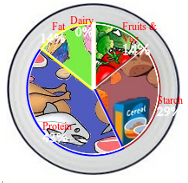
\epsfig{file=logbookapp.png, height=1.2in, width=1.4in}
\caption{An example of a meals' pie chart in the logbook app}
\label{figure:logbookapp}
\end{figure}
\begin{figure}
\centering
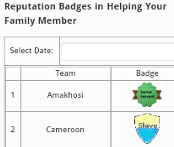
\epsfig{file=gameapp.png, height=1.2in, width=1.4in}
\caption{Examples of badges in a gamified app}
\label{figure:gameapp}
\end{figure}   
The experiment applied a ``within-group'' design of where, the same group of participants were exposed to different experimental conditions in to minimized the effect of confounding variables. In our case, examples of confounding variables that could be controlled with this experiment design are such as: variation in motivation levels of both beneficiaries, and intermediaries; technology operational skills of both beneficiaries , and intermediaries; education level of both beneficiaries; and beneficiaries; and etc. The advantage of using the ``within-group'' design is that it minimizes the sample size hence cutting down the cost of running experiments, and it also increases the power when using student t test with repeated measures. However by using this design approach another problem is introduced, and that is the learning effect. In order to minimize the impact of the learning effect on any experimental condition, each pair of users was randomly assigned to either one of the two experimental sequences (GL or LG groups). The LG group started with logbook and finished with gamification. The  GL group started with gamification and finished with logbook . Each group had 7 pairs of users. In this way the learning effects from the two experimental conditions are expected to cancel each other.  
\subsection{Data collection and Analysis} 
Prior to data collection each pair was given an android phone (Samsung
GT-S5300) installed with both a native link to a web app and native pedometer app. The phones were supposed to be handled by adults. We allocated 1.3 GB of data to use for 6 weeks. Also,each adult received ZAR 240 (approx. US \$20) as a compensation for transport and their time for the duration of the study. The data bundle was also an incentive to both members of a pair as they could use it for other purposes. \newline
The experiment lasted for 6 weeks (October 2015 to November 2015). For the first 4 weeks, the LG and GL groups were in logbook and gamification respectively. After switching, for the last 2 weeks, the LG and GL groups were in gamification and logbook respectively. The explanation of why four weeks in phase 1 and two weeks phase 2 is based on two reasons. Our plan was to divide time equally in three(3) weeks intervals, but phase one had extended to four(4) weeks instead of the three(3) weeks we had initially plan for and this was because we couldn't schedule a midline assessment immediately after the end of the third week since participants were not available hence we extended experimental switching until after the assessment. We also couldn't extend the experimental period in phase two to have the same number of days as phase 1 because it was approaching December and it was going to be tricky to gather participants as some would have travelled for holidays. In order to address this problem of inequality, when we assessed usage we only used a relative amount with respect to the number of days in which participants were given access to a particular experimental condition. This has no effect on either motivation to use any experimental condition since both logbook and gamification were both present in both phases. The effects on motivations due to different durations are expected to cancel each other.\newline
We collected data through a triangulation of usage logs, intrinsic motivation inventory(IMI) questionnaires, and interviews. We developed the IMI questionnaires with guidance of materials found on a ``Self-Determination Theory''\footnote{http://www.selfdeterminationtheory.org/intrinsic-motivation-inventory/} website which is maintained by researchers working on the theory including Richard Ryan and Edward Deci\cite{deci1985intrinsic} whom were early pioneers in developing the theory. These questionnaires were pretested in one of our early pilot studies.\newline
There were two sets of questionnaires, one for adults participants , and another one for children participants. Questionnaires were administered at three points: (1) baseline (before experiments); (2) midline (the fourth week, before switching of experimental conditions; (3) endline (after concluding usage experiment at the end of the sixth week).\newline
On questionnaire of children included sub-scales for the three basic psychological needs. Two more IMI questionnaires that assessed the overall motivations to self-monitor diet and activity included sub-scales that assesses basic psychological needs and in additional there were also sub-scales of, perceived effort, perceived usefulness, and perceived enjoyment.\newline 
Usage was measured by counting the number of sessions from each version of the system. A new session is defined as when an activity is detected in the absence of any activity in the past one hour or more. We computed the relative number of sessions since the number of days on which pairs of users spent on a particular experimental condition differ between LG and GL group. For instance the LG group spent nearly four weeks in logbook and two weeks in gamification while the GL group spent four weeks in gamification and two weeks in logbook. Therefore, we use number of sessions per day which is obtained using Equation \ref{equation:sessions}. Usage comparison between logbook and gamification excluded four pairs of users because they had various technical problems that hindered their full participation in both experimental conditions. The list of pairs that were excluded and reasons for their exclusion are summarised on Table \ref{table:usageproblems}.
\begin{equation}
\label{equation:sessions}
y=t\SB{i n}/d\SB{i n}
\end{equation}
where:\emph{y} is number of sessions per day, \emph{t\SB{n i}} is total number of sessions for pair ``n'' in experimental condition ``i'', and \emph{d\SB{n i}} is total number of days on which experimental condition ``i'' was available for pair ``n''.
\begin{table}[h!]
  \begin{center}
    \caption{Pairs with usability/technical problems that hinder their participation}
    \label{table:usageproblems}
	\begin{tabular}{|p{1cm}|p{0.8cm}|p{5cm}|}
		\hline
		Pair&Group&Problem\\
		\hline
		Pair A&GL &App not loading\\
		\hline
		Pair B&GL& Miss-allocation of data bundles.\\
		\hline
		Pair C & LG.& Pedometer never transmitted data.\\
		\hline
		Pair D & LG.& Pedometer stopped transmitting data.\\
	\hline
	\end{tabular}
  \end{center}
\end{table}
\section{Findings}
\subsection{Usage Trend} 
The usage of the app in a period of six weeks for all fourteen pairs is shown on Figure \ref{figure:usagedailysessions}.
\begin{figure}[htbp]
  \centering
    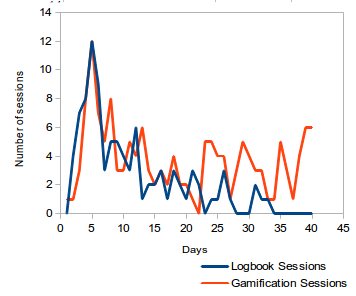
\includegraphics[width=0.35\textwidth]{scatter_daily_sessions.png}
    \rule{26em}{0.5pt}
  \caption{Total daily number of sessions from the two experimental conditions.}
  \label{figure:usagedailysessions}
\end{figure} 
Comparison of usage between logbook and gamification which excluded four pairs showed that the Log mean of number of sessions per day was significantly higher on gamification condition, M=0.459; SD=0.336, when compared to logbook condition, M=0.201 ;SD=0.196 with (t(9)= -2.6593 ; p= 0.0261 ; 95\% CI=  -0.477 to -0.039). We used log mean because we transformed the original data to have a normal distribution shape on the differences between number of sessions per day. What this finding suggests is that there was an indication of a significant increase in frequency of daily usage when pairs where in gamification condition.\newline
Another important finding on usage showed that the main logbook component functionality such as steps graphs, and diet charts had lower utilization during gamification condition compared to during logbook condition (Figure \ref{figure:self_monitoring_usage}).
\begin{figure}[htbp]
  \centering
    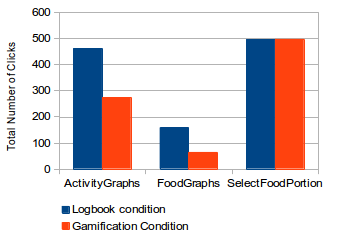
\includegraphics[width=0.35\textwidth]{self_monitoring_usage.png}
    \rule{26em}{0.5pt}
  \caption{Total clicks on main self-monitoring features: ``Logbook App'' versus ``Gamified App''.}
  \label{figure:self_monitoring_usage}
\end{figure}\newline
\begin{figure}[htbp]
  \centering
    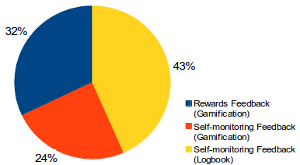
\includegraphics[width=0.3\textwidth]{clicks_distr.png}
    \rule{26em}{0.5pt}
  \caption{Distribution of clicks: self-monitoring features versus rewards features.}
  \label{figure:clicks_distr}
\end{figure}\newline 
This happens as intermediary participants paid more focus on virtual rewards which provided indirect feedbacks of steps and diet through badges, gardens etc. This is further supported by Figure \ref{figure:clicks_distr} which shows the distribution of clicks among feedback features of the ``Gamified Health App'' and the ``Logbook App''.
\begin{figure}[htbp]
  \centering
    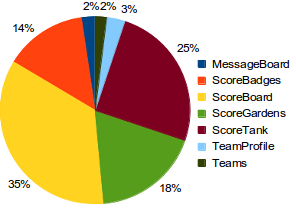
\includegraphics[width=0.32\textwidth]{clicks_rewards.png}
    \rule{26em}{0.5pt}
  \caption{Distribution of clicks in gamified features.}
  \label{figure:rewards_clicks}
\end{figure}
However, the trend in recording of diet/meals was almost similar between the two experimental conditions as the process of recording meals was instrumental in earning virtual rewards during gamification condition, therefore, intermediary participants continued to use the feature for recording during gamification condition. Utilization of gamification features showed highest usage on the leader board (scoreboard) as shown on Figure \ref{figure:rewards_clicks}.\newline
\subsection{User Experience of Intermediaries}
Most of the beneficiaries' app usage was facilitated by intermediaries  in proximate enabling and proximate translations. These types of intermediated interactions have been discussed in the work by Sambasivan et al.\cite{sambasivan2010}. The following factors influenced intermediaries to use the app : steps and diet feedbacks coupled with phone novelty effect; informal direct comparison on steps; virtual rewards; and requests from beneficiaries. Interest of intermediaries varied as some put value on the social relatedness brought by the intervention while others were concerned about achievements (i.e. dominating others in competitions).\newline
Despite higher frequency of usage in gamification condition reported above, the trend on average perceived enjoyment in logbook condition appears to be higher than in gamification condition for both age groups ( age \textgreater = median(15.5) or \textless 15.5) (Figure \ref{figure:PE_Interm_App_exp_seq}). The reason behind this trend is that not all intermediary participants had a positive user experience on utilizing gamification. We observed two factors that contributed  to this. The first factor is that there were pairs that had usage problems as we have seen on Table \ref{table:usageproblems} above. Among those four pairs, the user experience was severely bad in the intermediary users from pairs ``A'' and, ``C''.\newline
For pair A, the app demotivated the intermediary because it was not stable  and it was always failing to load and resulted into termination of usage after two days.\newline
For pair C, the pedometer never transmitted a single reading to the server but this pair continued to use the app throughout the logbook condition. An intermediary user from this pair was close to an intermediary from pair D which also experienced problems with pedometer but not so severe like for Pair C. Therefore, an intermediary user from pair C continued use the app although the steps never got transmitted to the server because of direct steps comparison. Steps for pair C could still be viewed directly from a native pedometer app as raw numbers. The two intermediary participants from pairs C, D shared their progress about steps walked by their respective beneficiary users whenever they met. This explained why the pedometer problem didn't affect the usage of the app by the intermediary user from pair C while in logbook condition. After pair C was switched to gamification, the inability of the pedometer to transmit steps to the server resulted to a negative user experience to the intermediary user from this pair. This also happened to pair D but it didn't affect much the motivation of this intermediary user as the pedometer was working until one week before switching of experimental conditions. Steps played a role in achievement of rewards. Intermediary user from pair C had done a lot of efforts with expectations that their pair will be rewarded once switched to gamification condition. This finding about expectations was shared by another intermediary user from pair E who was living close  to the two intermediaries from pairs C and D. She was concerned about the gamification system as she worried that the system was not fair because her peers had done more efforts compared to her but she was ahead of them and she didn't understand why was it the case. She was referring to what she had observed during logbook condition,  therefore she was expecting the efforts of her peers to transmute into rewards after they were both switched to gamification condition. As the result the problems on pairs C, D had a multiplier  effect on the perceived enjoyment of this intermediary user from pair E hence her motivation to use the gamified app and this affected her trust on the credibility of the gamified system.\newline 
\begin{figure}[htbp]
  \centering
    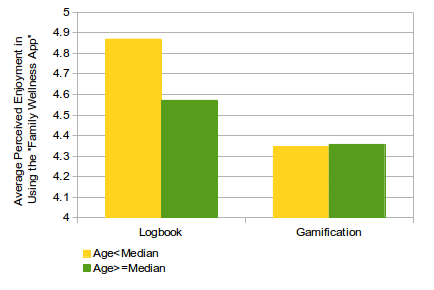
\includegraphics[width=0.35\textwidth]{PE_Interm_App_exp_seq.png}
    \rule{26em}{0.5pt}
  \caption{Intermediaries' average perceived enjoyment in using the app versus age group (Logbook and Gamification).}
  \label{figure:PE_Interm_App_exp_seq}
\end{figure}\newline
Gamification condition didn't harm motivation of only intermediary users with severe usability problems (from pairs A, C) as there was also another scenario on two other intermediary users from \textbf{Pairs F, } and \textbf{D}. These users had used the app more often while in gamification compared to when they were in logbook but had both reported lower scores in competence when they were in gamification compared to when they were in logbook. Upon reviewing their performance on gamification, it was observed that these two users never attained any advancement in badges despite their efforts during gamification. The reason for this is that their beneficiary users were not walking enough steps. As badges were earned in combination of both the app usage and average number of steps walked by a beneficiary user, then the absence of rewards harmed their enjoyment to use the gamified app. We attribute this negative experience to failure of our gamification system to match challenges with abilities as efforts of beneficiaries differed hence challenges didn't match with individual intermediaries' abilities.
\begin{table}[h!]
  \begin{center}
    \caption{Comparison of 10 intermediaries' scores on sub-scales of perceived competence (PC), perceived autonomy (PA), and perceived relatedness (PR) in using the ``Family Health App}
    \label{table:imiwellnessinterm}
	\begin{tabular}{|L{0.6cm}|L{3cm}|L{3cm}|}
		\hline
		Mean &Logbook&Gamification\\
		\hline
		 \multirow{2}{*}{PC}&M=5.23; SD=1.02&M=5.96; SD=0.66\\\cline{2-3} 

		 &\multicolumn{2}{|l|}{t(9)=-3.495; p=0.0068 ; 95\% CI= -1.204 to -0.258} \\
\hline
		 \multirow{2}{*}{PA}&M=3.95; SD=0.86&M=3.96; SD=0.94\\\cline{2-3} 

		 &\multicolumn{2}{|l|}{t(9)= -0.027; p= 0.98; 95\% CI= -0.596 to 0.582} \\
\hline

		 \multirow{2}{*}{PR}&M=4.22; SD=0.63&M=4.37; SD=0.9\\\cline{2-3} 
		 &\multicolumn{2}{|l|}{t(9)= -0.719; p=0.49; 95\% CI= -0.622 to 0.322 } \\
\hline
	\end{tabular}
  \end{center}
\end{table}
\newline
We then compared the ability of the two versions of the app to afford the three basic psychological needs. In this comparison we excluded pairs A, C, F, and G due the reasons we have stated above. The results for this comparison is shown on Table \ref{table:imiwellnessinterm}. Perceived competence of intermediaries in using the ``Family Health App'' was significantly higher in the gamified condition than in the logbook condition. This means a gamified system gave intermediary users challenges and these challenges motivated an increase in frequency of using the app. There were no significant differences on both perceived autonomy and relatedness. 
\subsection{User Experience of Beneficiaries} 
Since most beneficiaries only interfaced with the app through intermediary users, beneficiaries' user experience relied on cooperation they got from intermediaries. Young beneficiary participants appeared to follow what was happening in gamification but this interest diminished with age. In some situations beneficiary users  had negative experience, especially when they needed help and intermediary participants felt as if they were being bothered.\newline
We also compared the overall impact of the app on motivation to self-monitor diet and activity at baseline, midline, and endline. We used the IMI questionnaire with six sub-scales; perceived competence, perceived autonomy, perceived relatedness, perceived enjoyment,  perceived usefulness, and perceived effort. The overall IMI scores were computed by averaging scores from individual sub-scales. Only ten beneficiary participants were considered for analysis. Four were excluded because of usage problems in their pairs highlighted on Table \ref{table:usageproblems} above as these problems affected the ability to self-monitor.
\begin{table}[h!]
  \begin{center}
    \caption{Comparison of 10 beneficiaries' IMI scores in diet self-monitoring (baseline, midline,endline}
    \label{table:imidietbenf}
	\begin{tabular}{|L{3.3cm}|L{1.1cm}|L{1.1cm}|L{1.1cm}|}
		\hline
		Mean IMI Score &Baseline&Midline&Endline\\
		\hline
		 %\multirow{3}{*}
		 {Self-monitoring of Diet}&M=4.48; SD=1.24&M=5.07; SD=1.19;&M=5.55; SD=0.95\\\cline{2-4} 

		&\multicolumn{3}{|l|}{F(2,18)=3.787; p=0.042} \\
\hline	\end{tabular}
  \end{center}
\end{table}
\begin{figure}[htbp]
  \centering
    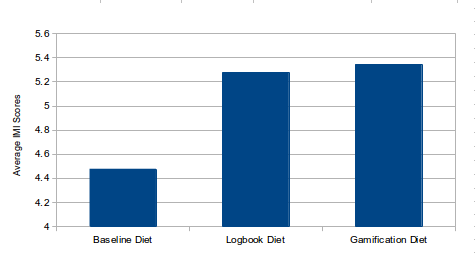
\includegraphics[width=0.4\textwidth]{imi_diet2.png}]
    \rule{26em}{0.5pt}
  \caption{Trend on average IMI scores of self-Monitoring of diet at baseline, logbook, and gamification.}
  \label{figure:imi_diet2}
\end{figure}\newline
The results of one way ANOVA with repeated measures on self-monitoring of diet (baseline, midline, and endline)(Table  \ref{table:imidietbenf}) showed  a significant time effect on average IMI scores. Pairwise comparisons with a paired student t-test indicated that the average score was significantly higher at endline when compared to baseline (t(9)=-2.457; p=0.036; 95\% CI= -2.06083 to -0.08517 ). There were no significant differences between midline and baseline (t(9)=-1.298; p=0.227 ; 95\% CI= -1.621 to 0.439), and between midline and endline (t(9)=-1.975; p=0.08 ; 95\% CI= -1.0342 to 0.07017). The performances of Logbook and gamification appear to be the same.\newline
We conducted another analysis (N=9) to examine if there is a difference among baseline,midline, and endline in self-monitoring of activity. The sample size was now 9 because one participant didn't complete the questionnaire. ANOVA (Table \ref{table:imiactivitybenf}) showed that there was no significant difference of average IMI scores on self-monitoring of activity measured at baseline, midline and endline. The trend of means appears to increase from baseline to endline as shown on Figure \ref{figure:imi_activity}. Also for activity, the trend of gamification and logbook are almost similar.
\begin{figure}[htbp]
  \centering
    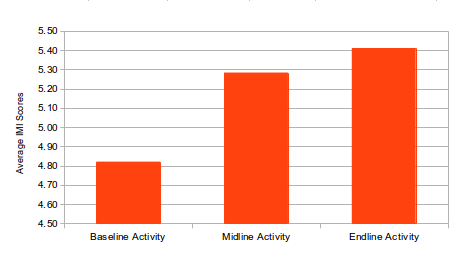
\includegraphics[width=0.4\textwidth]{imi_activity.png}
    \rule{26em}{0.5pt}
  \caption{Trend on average IMI scores of self-monitoring of activity at baseline, midline, and endline.}
  \label{figure:imi_activity}
\end{figure}
\begin{table}[h!]
  \begin{center}
    \caption{Comparison of ten beneficiaries' IMI scores in self-monitoring of activity at baseline, midline and endline}
    \label{table:imiactivitybenf}
	\begin{tabular}{|L{2.5cm}|L{1.3cm}|L{1.3cm}|L{1.5cm}|}
		\hline
		Mean IMI Score &Baseline&Midline&Endline\\
		\hline
		 %\multirow{3}{*}
		 Self-monitoring&M=4.82; SD=1.002&M=5.28; SD=1.003&M=5.41; SD=0.894\\\cline{2-4} 
		 of activity&\multicolumn{3}{|l|}{F(1.182, 9.455)=2.936; p=0.116} \\
\hline	\end{tabular}
  \end{center}
\end{table}
\section{Discussion}
Findings have indicated that gamification has a tendency of increasing daily frequency of usage. Also intermediaries are likely to feel more competent during gamification condition. In addition, gamification is not different from logbook in motivation of beneficiaries as perceptions of beneficiaries towards self-monitoring of activity and diet using the two versions of the system are not different. However, the intervention in general appears to significantly increase the motivation of beneficiary users to self-monitor diet at endline when compared to baseline. The trend is also similar in self-monitoring of activity although it was reported not to be statistically significant. We report on some design implications that are important in motivation to engage with the app.
\subsection{Factors on Usage Motivation}
The app was mostly used by intermediary participants. There are some variation of external factors that mediated usage among intermediary participants. These variations can inform how one need to design an app for this usage context. These factors may not be independent of each other as there may be some interactions between factors.
\subsubsection*{\textbf{Playfulness  of the Self-monitoring Task}} 
The task itself without rewards showed the capability to invoke interests of intermediary and beneficiary users. Phrasing the intervention by suggesting the notion of an intermediary managing the wellness of a beneficiary participant can create a room for playfulness behaviours when the two users from a pair interact. An intermediary can become curious of how many steps have been walked by a beneficiary participant and this will lead to the two users conversing in a playful manner depending on how the two users are excited about the information presented. Therefore, this feature is important as it can motivate ongoing usage for members of a pair and its effectiveness may depend on the strength of the bond that already exists between the two users or improvement of relatedness between the two users of a pair as the result of using a self-monitoring feature. Self-monitoring is an important feature that is suggested in any persuasive technology \cite{Oinas-kukkonen:psd}. Therefore, in our context one can take advantage of bonding between family members to sustain an ongoing use of a personal health informatics through intermediaries.  
\subsubsection*{\textbf{Laveraging Sharing of Phones}}
The phenomenon of sharing phones is important in our context. Parents were lending their phones to their kids to access social media sites and games. Having access to a phone while providing help to beneficiary participants can be viewed as one of the motivating factors to intermediary participants who didn't have smart-phones or data bundles in their smart-phones. Some intermediary participants had installed games, other apps on those phones. In the context of ICTD, non-prescribed use of devices or other technologies allocated for an intervention is considered to be an aspect of play which is a capability as it fosters motivation to participate in an intervention \cite{ferr2015:play}. Therefore, one can capitalize on this motivation introduced as the result of sharing phones and it can be viewed as part of motivational affordances to encourage ongoing use of a system through young intermediaries within family settings.
\subsubsection*{\textbf{Support for Steps/Diet Comparisons}}
Direct comparison of steps/diet needs to be supported within the app context as it has a potential to increase engagement of both intermediary and beneficiary users. A study by ''Anonymized'' et al \cite{katule2016:leveraging} found this form of comparison to be more interesting to beneficiary users compared to gamification features. The most interesting phenomenon in their work was that the comparison was informal as it was not supported within user interfaces. Therefore, beneficiary participants utilized SMS or face to face interactions as they lived nearby.\newline
In the findings of this paper, informal comparisons of steps were also common in our context, except in our study they were also carried out by intermediary participants especially those who where from pairs in logbook condition. This was common for intermediaries who were close or living nearby, and in some cases it happened in the absence of gamification. This entailed comparing of steps walked by their respective beneficiary participants. However, the interest of intermediaries changed the moment virtual rewards were introduced (Figures \ref{figure:self_monitoring_usage} and \ref{figure:clicks_distr} above). The objective of a personal health informatics system is to support reflective learning, therefore, it is important to provide software support for direct comparison of steps or diet as this information is more meaningful to beneficiary participants compared to game design mechanics such as points which are well understood by intermediary participants only. This is one of the ways to increase engagement of beneficiary users especially the older ones who are likely to be less interested with game mechanics. It is also anticipated that direct comparison of steps and diet will increase interest of intermediary participants on steps graphs and diet charts as this form of comparison will entail some form of competitions. This can encourage intermediary users to share information with their beneficiary users and even persuade them instead of more focus being directed on virtual rewards.
\subsubsection*{\textbf{Game Design Elements}} Availability of game design elements increased the frequency of intermediary users checking the app during the day. Interests on game elements varied as some participants were motivated by achievements while others showed the desire to interact with others by commenting on their fitness gardens, and aquariums. This variation in interests exhibits differences in intermediary users' traits. The importance of tailoring persuasive games according to personalities of players has been emphasized\cite{orji2013:tailoring}. For instance Arteaga \cite{arteaga2010:persuasive} designed a study involving motivating teenagers to exercise using persuasive health games, each player selected a game that matches their personality. To support this idea, one could give more autonomy on intermediary users, to select which features they would like to include in their interfaces from a range of features such as chat rooms, leader-boards, botanical gardens etc. More autonomy can also be given in customization of privacy in terms of whether they would like to share their information or not. Customization of avatars is also important because we observed that most users changed their avatars during gamification and one user explained that she sees the avatar she selected as a representation of herself. Through avatars, these users embodied their identities. Allowing users to create or change avatars in an example of how an ICT system can afford autonomy \cite{zhang2008:motivational}
\subsubsection*{\textbf{Request from Beneficiaries}}  
Usage can also be influenced by requests from beneficiary users who might also be influenced by  aforementioned factors. Therefore, this usage influence could start by an external reward such as perceived usefulness or social comparison and then this leads to a beneficiary user passing a request to an intermediary user. There were times where intermediary users engaged with the app only upon receiving requests from beneficiaries.  We observed cases of where intermediary participants autonomy was violated as requests came at the time where intermediary participants were either studying for exams or doing something else and they felt it was not the right time to fulfil those requests. This made intermediary participant to feel that their parents were nagging them. Therefore, it is important to foster motivation of intermediary users through tailored motivational affordances in order to increase intermediary users' autonomy\newline
\subsection{Matching Gamification to Skills}
In addition to factors on usage motivation, we also discuss the use of gamification in particular. There were negative experiences in  gamification as it  appeared to harm intrinsic motivation of some intermediary users. Awarding virtual rewards to intermediary users based on partial efforts from beneficiary participants seemed not to resonate with the notion of matching challenges to skills of the main users. For instance in awarding badges there were two conditions to be met. The first condition was that the app has to be used for a certain minimum number of days as specified by requirements of a specific badge. The second condition was that, an average number of steps that have been walked so far has to be not below a certain threshold for that specified badge. It became impossible for some intermediary users to move from one badge to the next because efforts by beneficiary users differed and this may impacted motivation of intermediary participants. When challenges are too difficult as they don't match users' skills, end users can become demotivated \cite{zhang2008:motivational}.\newline 
We propose approaches that could be used to curb the effect of the  aforementioned shortcoming. First is to allow users to select different levels of gamification they want to participate. There could be levels such as beginners, intermediate, advanced, etc. Pairs that are on the same level could be grouped together and not mixed with pairs with levels that are different. The second approach is to allow intermediary participants to benefit from the app information, by incorporating their wellness data i.e. steps. The former can also be combined with the latter. There were some observed scenarios that support the utilization of the latter approach. For instance, there was one pair of whereby not only the beneficiary participant was using the pedometer as an intermediary was also using it. They were taking turns to use the pedometer, therefore, they were collaborating in accumulating steps. This pair had discussions of whether the person whose turn it was had walked enough steps. The goal was to accumulate more steps than other pairs. A different scenario is whereby intermediaries claimed to also be benefiting from nutrition/diet information since the same type of meal is shared at home, therefore, if beneficiary participants ate something that is not healthy while at home then there is a likelihood of an intermediary participant to have eaten the same type of meal too.
\section{Conclusions}
Gamification and other motivational affordances brought by factors such as self-monitoring, social comparison, and sharing of phones have potentials to increase engagement of young intermediary users to assist adult beneficiary users in interacting with a personal health informatics. More time should be spent on designing a system that give more autonomy to intermediary users and reduces negative experiences with a pair of users. Such a system can increase usage of a personal health informatics to beneficiary users who are inexperience with technology. This study has demonstrated that it is feasible to utilize various motivational affordances to design a system that motivate on going use through intermediary users. Our study is limited in sample size and also some of the design recommendations should be tested in the field by future studies. In addition we faced a myriad of challenges affect generalizability of these findings. Ramachandran and Goswami~\cite{ramachandran2010research} have also highlighted how doing research in ICTD context poses challenges to the rigour of research design. This one step towards facing the feasibility of engaging intermediaries through gamification. There are many unexplored issues such spatial arrangement of technology and users; i.e an optimal arrangement for technology design to support flow to both intermediaries and beneficiaries, comparison between using intermediaries and without intermediaries.


In addition, future studies could also explore on interaction between factors that influenced usage.  
%\end{document}  % This is where a 'short' article might terminate

%ACKNOWLEDGMENTS are optional 

%\section{Acknowledgments} 

%
% The following two commands are all you need in the
% initial runs of your .tex file to\ref{equation:sizetrees}
% produce the bibliography for the citations in your paper.
%small{
\bibliographystyle{abbrv}
\bibliography{sigproc} %} % sigproc.bib is the name of the Bibliography in this case
% You must have a proper ".bib" file
%  and remember to run:
% latex bibtex latex latex
% to resolve all references
%
% ACM needs 'a single self-contained file'!
%
%APPENDICES are optional
%\balancecolumns

\end{document}